
%(BEGIN_QUESTION)
% Copyright 2015, Tony R. Kuphaldt, released under the Creative Commons Attribution License (v 1.0)
% This means you may do almost anything with this work of mine, so long as you give me proper credit

\noindent
Identify which protective relays in this system will trip breakers in the event of the following faults:

\begin{itemize}
\item{} A tree branch touching one of the power line conductors feeding Load B
\vskip 10pt
\item{} An internal phase-to-phase fault inside circuit breaker 4
\end{itemize}

$$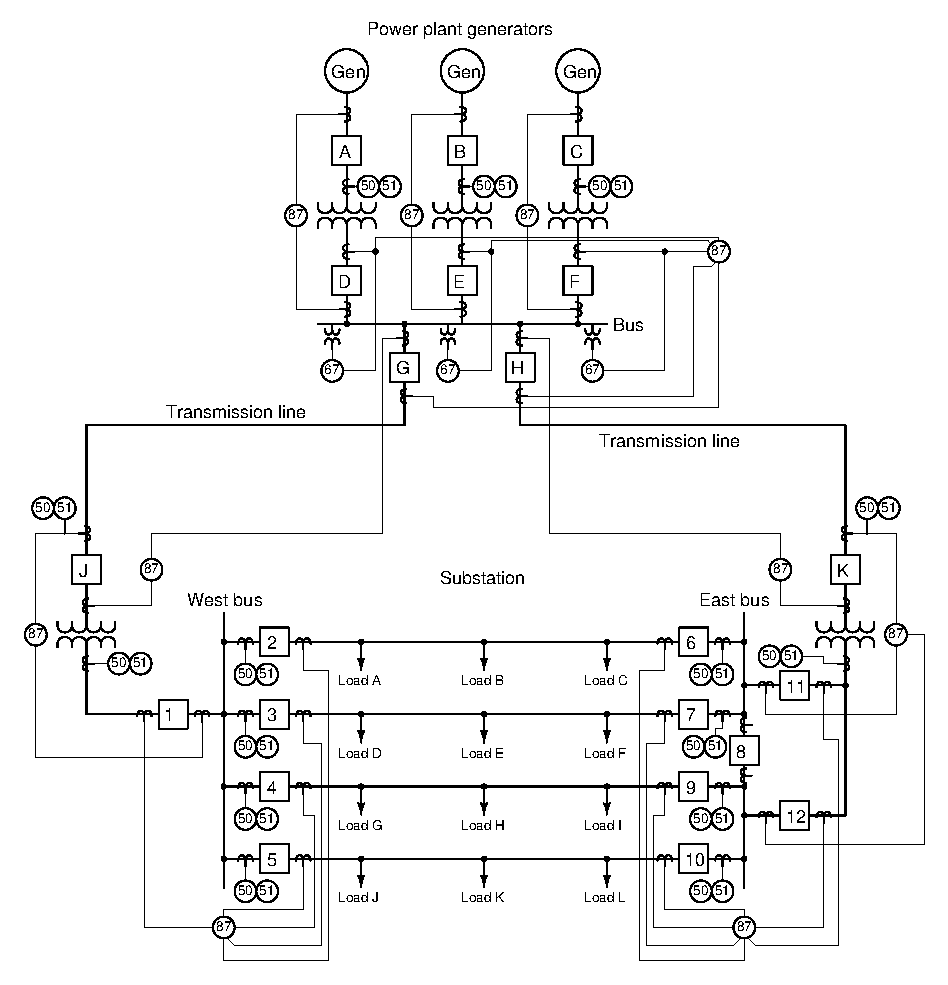
\includegraphics[width=15.5cm]{i02878x01.eps}$$

\underbar{file i02878}
%(END_QUESTION)





%(BEGIN_ANSWER)

\begin{itemize}
\item{} A tree branch touching one of the power line conductors feeding Load B: {\it one of the overcurrent relays (50 or 51) at breaker 2 and/or breaker 6 depending on which of those two breakers is closed}
\vskip 10pt
\item{} An internal phase-to-phase fault inside circuit breaker 4: {\it the 87 (differential) relay immediately the West substation bus} 
\end{itemize}

Award partial credit (2 points) for the second answer if it cites one of the overcurrent relays monitoring breaker 4's current, rather than the differential relay which will be faster-acting.

%(END_ANSWER)





%(BEGIN_NOTES)

{\bf This question is intended for exams only and not worksheets!}.

%(END_NOTES)


